% !TEX encoding = UTF-8 Unicode
% !BIB TS-program = biber
%
% This file is MIT-Thesis.tex, a LaTeX template for formatting an MIT thesis with the mitthesis class.
%
% Version: 1.20, 2025/05/02
%
% Author: John H. Lienhard, copyright 2025. Reuse under the MIT license: https://ctan.org/license/mit 
%
% Documentation is here: https://ctan.org/pkg/mitthesis


%% Don't modify the \DocumentMetadata command unless you know what it does. 
%% If this command throws an "undefined" error, your latex installation is out of date: try commenting this command out.
\DocumentMetadata 
{
	lang		= en-US,
	pdfversion  = 1.7,
	pdfstandard = a-2b,
%	debug		= {xmp-export}, % if you want to check your metadata (xmpi file).
}

%%%%%%%%%  Documentclass and options  %%%%%%%%%%%%%%%%%%%%%%%%%%%%%%%%%%%%%

\documentclass[twoside]{mitthesis}% fontset=libertinus, fontset=lmodern, fontset=lucida, 
%						fontset=fira-newtxsf, fontset=newtx, fontset=newtx-sans-text,  
%						fontset=heros-stix2,  fontset=stix2, fontset=termes-stix2, fontset=termes
%
% option [twoside]		gives facing-page behavior for printing; omitting twoside will eliminate even-numbered blank pages.
%
% option [lineno]	 	provides line numbers, as for editing
%
% option [fontset=xxx]  is a keyvalue which can be:
%					 	for pdftex or lualatex engine:  defaultfonts, libertinus, lmodern, lucida
%					 	for pdftex only: 				fira-newtxsf, newtx, newtx-sans-text
%						for lualatex only:				heros-stix2, stix2, termes, termes-stix2
%					 	if no key value is given, fonts default to CMR (pdftex) or LMR (unicode), i.e., "the LaTeX font".
%					 	You can edit the fontset files or you can write your own, myfonts.tex, and do [fontset=myfonts].
%						If you are using multiple languages, load the babel package in your fontset file, before the fonts.
%
% option [mydesign] 	loads packages for color, title and list formats, margins, or captions. 
%	or [mydesign=file]	You can edit mydesign.tex to change defaults. Other design files can be loaded as
%						key values, [mydesign=filename], where filename.tex should be in your working directory.
%						Two example files are provided: mydesign_redsans_headings.tex and mydesign_libertinus_headings.
%						See documentation for details and a description of the appropriate fontsets to use with each.						

%%%%%%%%  Packages used in sample chapters (not otherwise required) %%%%%%%

%% Package for code listing in Appendix A.
\usepackage{listings}%   documentation is here https://ctan.org/pkg/listings

%% Set chemical formulas nicely
\usepackage[version=4]{mhchem}%   documentation at https://ctan.org/pkg/mhchem

%% Latin filler used in Chapter 1, with a test for package version date (https://ctan.org/pkg/lipsum)
\usepackage{lipsum}
\IfPackageAtLeastTF{lipsum}{2021/09/20}{\setlipsum{auto-lang=false}}{}


%%%%%%%%%  Other optional packages used sample chapters  %%%%%%%%%%%%%%%%%%

%% Table related packages  

\usepackage{booktabs}% publication quality tables (https://ctan.org/pkg/booktabs)

\usepackage{array}% Additional options for column formats (https://ctan.org/pkg/array)

\usepackage{dcolumn}% For alignment of numbers on the decimal place (https://ctan.org/pkg/dcolumn) 
  \newcolumntype{d}[1]{D{.}{.}{#1}}% use with dcolumn package. Note: dcolumns are set in math mode.
  % syntax: d{x.y} where x is max number of digits before decimal and y is max number after.

% Package for multipage table in Appendix B.
\usepackage{longtable}% typeset multi-page tables (https://ctan.org/pkg/longtable)

%\usepackage{tabularx}% adjustable-width columns in tabular (https://ctan.org/pkg/tabularx)


%% Package for improved typography
\usepackage{microtype}% typographic fine-tuning (https://ctan.org/pkg/microtype)


%% Load this if using the two-column nomenclature format, \begin{nomenclature*}
\usepackage{multicol}

% Hannah (me) added
\usepackage{xspace}


%%%%%%%%%  Graphics path (to figure files)  %%%%%%%%%%%%%%%%%%%%%%%%%%%%%%%%

%% Can set graphicspath to point to specific directories containing figures (the current directory is searched automatically)
%% For instance, to search a subdirectory of the current directory called "figures" and a parallel directory called "art", set:

% \graphicspath{ {figures/} {../art/} }% For details see: https://latexref.xyz/dev/latex2e.html#g_t_005cgraphicspath


%%%%%%%%%  Representative set-up for biblatex  %%%%%%%%%%%%%%%%%%%%%%%%%%%%%

%% biblatex is very powerful, and you can customize most aspects the reference list and citations to suit your needs.
%%   documentation is here: https://ctan.org/pkg/biblatex
%%   cheat sheet is here:   https://tug.ctan.org/info/biblatex-cheatsheet/biblatex-cheatsheet.pdf

%% Numerical citations of references
\usepackage[style=ext-numeric-comp,giveninits=true,maxbibnames=10,sorting=none,language=american]{biblatex}

% and make some changes to that style
	\renewcommand{\multicitedelim}{\addcomma}% removes space between consecutive cites to give [6,7], not [6, 7]
    \AtEveryBibitem{%
      \ifentrytype{article}{%
        \renewbibmacro{in:}{}% Removes "In:" for articles
		\renewcommand*{\jourvoldelim}{\addcomma\space}   % put comma after journal title
		\renewcommand*{\volnumdatedelim}{\addcomma\space}% put comma after volume info
		\renewbibmacro*{issue+date}{% Print date without parentheses around it
		\iffieldundef{issue}%
        	{}%
        	{\printfield{issue}%
         	\setunit*{\addcomma\space}
        	}%
			\printdate
		}
      }{}
    }
	\renewbibmacro*{volume+number+eid}{%
        \printtext[bold]{\printfield{volume}}%    bold volume (issue number) , eid
        \printtext[parens]{\printfield{number}}%  
        \setunit{\bibeidpunct}%
        \printfield{eid}
    }



%% IEEE style citations and references
% \usepackage[style=ieee,maxbibnames=10,sorting=none]{biblatex}% style=ext-numeric-comp,articlein=false,giveninits=true
%	 \DefineBibliographyStrings{english}{url= \textsc{url} ,  }% replaces the IEEE default "[Online]. Available" by "URL"

%% author-year style citations and references 
%% use \parencite, not \cite, when you want "(Author, year)"
%% The sample files are not set up to include parentheses.
% \usepackage[style=authoryear, maxbibnames=10]{biblatex} 


\addbibresource{mitthesis-sample.bib}%% <== change to YOUR bib file <= CHANGE


%% to avoid split urls and stretched white space, you can make the bibliography ragged-right by uncommenting this:
%\AddToHook{cmd/bibsetup/after}{\raggedright}

%% To ensure citations are set, run Latex --> biblatex --> Latex again (unless you installation does this automatically)


%%%%%%%%%%  Option for "double spacing" %%%%%%%%%%%%%%%%%%%%%%%%%%%%%%%%%%%%

%% Back in the typewriter era, double spaced lines were convenient for editing with a pencil. 
%% In typography, the separation between lines is called "leading", and it is usually set in 
%% proportion to the font size (i.e., when the font is loaded).  If you really feel the need 
%% to change the line separation, the most attractive results will be obtained by changing the
%% leading in proportion to the the current font size, rather than just doubling the space.

%% The setspace package provides a tool for changing line separation. Use these two commands here:
%
% \usepackage{setspace}%  documentation at https://ctan.org/pkg/setspace
% \setstretch{1.1}% you can choose some other value for the stretch of space between lines
%
%% Use one or more of the these commands *AFTER* the frontmatter
%
% \onehalfspacing
% \doublespacing
% \singlespacing  % will turn these effects off (you can use these anywhere in the document)

%% The best result is usually to stay with the default leading (or to learn about latex font settings).


%%%%%%%%%%%  Metadata  %%%%%%%%%%%%%%%%%%%%%%%%%%%%%%%%%%%%%%%%%%%%%%%%%%%%%%%

% Most of the document metadata is created automatically. 
% The following items should be adjusted to match your work. <================= !!!!!!!!!!

\hypersetup{%
	pdfsubject={Template for writing MIT theses with the mitthesis class},
	% Change this to briefly state topic of your thesis 
% 
	pdfkeywords={Massachusetts Institute of Technology, MIT},
	% Add keywords that will help search engines and libraries to find your work.
	% Includes the name[s] of the author[s] 
	% (If you used \DocumentMetadata at line 14, you can just put "\CopyrightAuthor," for the names.)
%
	pdfurl={},
	% If you have a url for the thesis, put it here. Otherwise delete this.
	% (MIT Libraries will put your thesis in DSPACE with a persistent url after you submit it.)
%	
	pdfcontactemail={},
	% You can put a [permanent] email address into the metadata, if you like.
	% Otherwise delete this.
%
	pdfauthortitle={},
	% If you have a title (e.g., Prof. Dr.-Ing.), you can include it here.
}

%%%%%%%%%%%%  Math operators %%%%%%%%%%%%%%%%%%%%%%%%%%%%%%%%%%%%%%%%%%%%%%%%%%%%

% These commands declare two math operators, \erf{..} and \erfc{..} using mathtools
% note: * form produces automatic delimiter scaling; optional argument sets size manually, e.g. [\bigg]
% See Table 1.1 in Chapter 1

\newcommand{\schedidle}{\texttt{sched\_idle}}
\newcommand{\schednormal}{\texttt{sched\_normal}}
\newcommand{\cgroups}{\texttt{cgroups}}

\newcommand{\eg}{{e.g.},\xspace}
\newcommand{\ie}{{i.e.},\xspace}

\newcommand\hmng[1]{\textcolor{blue!40!red}{[hmng: {#1}]}}


%%%%%%%%%%%%%%  End preamble %%%%%%%%%%%%%%%%%%%%%%%%%%%%%%%%%%%%%%%%%%%%%%%%%%%%%%%%%%%%%%%%%%%%%
%%%%%%%%%%%%%%%%%%%%%%%%%%%%%%%%%%%%%%%%%%%%%%%%%%%%%%%%%%%%%%%%%%%%%%%%%%%%%%%%%%%%%%%%%%%%%%%%%%

\begin{document}
%%% edit the following commands to match your thesis %%%%%%%%%%

\title{Modifying Linux to separate best effort from latency critical workloads}

% \Author{Author full name}{Author department}[Author's first PREVIOUS degree][Author's second PREVIOUS degree][...
% Note that third, fourth, fifth, and sixth arguments are optional [] and may be omitted

% note on names: most of the following names are made up; Silas Holman was a physics professor at MIT in the 19th century.

\Author{Hannah Manuela Nelle Gross}{Department of Electrical Engineering and Computer Science}

% Use once for each degree fulfilled by thesis
% For two degrees from one department, leave the department argument blank for the second degree {}.
\Degree{Master of Science}{Department of Electrical Engineering and Computer Science}
%\Degree{Bachelor of Science in Mechanical Engineering}{Department of Mechanical Engineering}

% If there is more than one supervisor, use the \Supervisor command for each.
\Supervisor{M. Frans Kasshoek}{Professor of Computer Science}

% Professor who formally accepts theses for your department (e.g., the Graduate Officer, Professor Sméagol,...)
% If more than one department, use more than once
\Acceptor{TODO TBD}{Professor of Probably Something}{Graduate Officer, Department of Research} % \\ \> Third title}
% \Acceptor{Quarta Castor}{Professor of Lodge Building}{Graduate Officer, Department of Mechanical Engineering}
%%%  If you need to reduce vertical space, put the acceptor title in the second argument and leave the third blank, {}.
% \Acceptor{Primus Castor}{Professor and Undergraduate Officer, Department of Physics}{}

% Usage: \DegreeDate{Month}{year}
% Valid degree months are February, May, June, or September
\DegreeDate{September}{2025}

% Date that final thesis is submitted to department
\ThesisDate{August 15, 2025}


%%%%%%  Choose whether to have a CREATIVE COMMONS License  %%%%%%%%%%%%%%%%%%%%%%%%%%%%%%%%%%%%%%
%
% If you are using a cc license, uncomment the following line and insert details of your cc license here.
%
% \CClicense{CC BY-NC-ND 4.0}{https://creativecommons.org/licenses/by-nc-nd/4.0/}
%

%%%%%%%  Solutions for overflowing titlepage  %%%%%%%%%%%%%%%%%%%%%%%%%%%%%%%%%%%%%%%%%%%%%%%%%%%

% If your title page is overflowing (from too many names, degrees, etc.):
%
% (a) you can reduce the 12pt and 18pt skips between various blocks to 6pt with this command:
%
% \Tighten
%
% (b)  you can scale down the Signature block at the bottom with this command:
%
% \SignatureBlockSize{\small}  %or this one \SignatureBlockSize{\footnotesize}
%
% (c) you can put the acceptor name and title onto two lines, rather than three like this:
%
% \Acceptor{Tertius Castor}{Professor and Graduate Officer, Department of Research}{}
%
% (d) you can change the font size of the author name[s] with
%
%	\AuthorNameSize{\normalsize}
%
% (e) and you can omit any previous degrees from the title page, instead mentioning them in the biographical sketch

% Also, if you prefer to keep the text toward the top of the page with most white space at the bottom, you
% can use this command to squash all of the vertical glue (stretchy space) with this command:
%
% \Squash 
%
% This command is useful when the text has not already reach the bottom of the page, since the glue gets squashed automatically
% when the page is too full.

%%%%%%%%%%%%%%%%%%%%%%%%%%%%%%%%%%%%%%%%%%%%%%%%%%%%%%%%%%%%%%%%%%%%%%%%%%%%%%%%%%%%%%%%%%%%%%%%%


%%% Make titlepage
\maketitle


%%%%%%%%% Content that you need to write follows! %%%%%%%%%%%%%%%%%%%%%%%%%%%%%%%%%%%%%%%%%%%%%%

% \includeonly{acknowledgments,biography,chapter1,chapter2,...,appendixa,...} 
%   for usage of includeonly, see https://latexref.xyz/_005cinclude-_0026-_005cincludeonly.html


%%% Frontmatter (write this material in the mentioned files)  %%%%%%%%%%%%%%%%%%%%%%%%%%%%%%%%%%%

% % Sample thesis committee page for mitthesis.cls
% Version 1.03, 2025/05/01
%
% This page is not required by the MIT Libraries, but some departments require it.
%
% Insert between title page and abstract page.
% Format this page in any way that you like (no specific requirements exist)
% 
% Add supervisor titles, degrees, and departments as appropriate, starting at line 32.


%%%%%  Formatting commands (you can ignore these)  %%%%%%%%%%%%%%%%%%

%% format this chapter title
\newcommand\CMstyle[1]{\pdfbookmark[0]{#1}{thesiscommittee}\bfseries\Large\lsstyle \MakeUppercase{#1}}

\newcommand\CMsubstyle[1]{\pdfbookmark[1]{#1}{#1}\flushright\normalfont\scshape\large\lsstyle #1}

%   \lsstyle produces additional letter separation (appropriate for capitalized display text),
% 	when \usepackage{microtype} has been given in the preamble. 
% 	If microtype has not been loaded, mitthesis.cls will ignore this command.
% 	The extra space added between letters is 100/1000 em (adjustable, see microtype documentation).


%%%%%%%%%%  EDIT THE NAMES AND TITLES IN THIS PART  %%%%%%%%%%%%%%%%%%%%%%%%%%%%%%%%%%%

\chapter*{\CMstyle{Thesis Committee}}

\section*{\CMsubstyle{Thesis Supervisor}}
\begin{flushright}

 \textbf{Marcus Gavius Apicius} \\ %% <======= edit these lines! 
 {\itshape
  Professor of Cooking Arts \\
  Department of Food Science \\
 }

\end{flushright}


\section*{\CMsubstyle{Thesis Readers}}
\begin{flushright}

 \textbf{Marie-Antoine Carême} \\ %% <======= edit these lines! 
 {\itshape
   Professor of Haute Cuisine \\
   Department of Food Science \\[18pt]
 }

 \textbf{Julia Child} \\ %% <======= edit these lines! 
 {\itshape
   Professor of French Cuisine \\
   Department of Food Science \\[18pt]
 }

 \textbf{Miles Gloriosus} \\ %% <======= edit these lines! 
 {\itshape
   Professor of Personal Pronouns \\
   Department of Rhetoric \\
 }

\end{flushright}
% This page is optional. Edit the file committee_members.tex 

% The abstract environment creates all the required headings and footers. 
% You only need to the text of the abstract in the file abstract.tex
\begin{abstract}
	\begin{abstract}
    
Widely-used container orchestration systems like Kubernetes are surprisingly
unable to honor the reservations of LC applications in the presence BE
workloads: a Kubernetes web application's mean latency jumps from 6.2ms to
$\sim$13ms after starting a BE image resize job. This paper traces this problem
down to Linux's cgroups, and show that because Linux uses per-core runqueues,
its weight-based interface is not enforced across cores.

This paper proposes an API that separates best effort workloads from critical
ones with reservations by introducing the BeClass priority class. BeClass
requires fewer cross-core interactions than a weight-based approach, and ensures
that no BE is ever running when an LC is queued. During high load this requires
`parking', which enforces that BEs user-space code doesn't run if doing so would
interrupt an LC process, but continues to run kernel-level services for the BE
so that when load goes down it can continue to run.

Experiments with a BeClass implementation in Linux show that BeClass ensures LC
processes' access to their reserved cores, while running BE workloads
opportunistically. When using BeClass in the same Kubernetes experiment, the
application's mean latency stayed stable at 6.2ms even after starting the BE.

\end{abstract}
% use \input rather than \include because we're inside an environment
\end{abstract}

%% acknowledgments.tex

% From mitthesis package
% Version: 1.02, 2024/06/19
% Documentation: https://ctan.org/pkg/mitthesis

\chapter*{Acknowledgments}
\pdfbookmark[0]{Acknowledgments}{acknowledgments}


Write your acknowledgments here.
% acknowledgments.tex (.tex extension is presumed by \include) 

% %% biography.tex
%% This section is optional

% From mitthesis package
% Version: 1.02, 2024/06/19
% Documentation: https://ctan.org/pkg/mitthesis

\chapter*{Biographical Sketch}
\pdfbookmark[0]{Biographical Sketch}{biosketch}


Silas Whitcomb Holman was born in Harvard, Massachusetts on January 20, 1856. He
received his S.B. degree in Physics from MIT in 1876, and then joined the MIT
Department of Physics as an Assistant. He became Instructor in Physics in 1880,
Assistant Professor in 1882, Associate Professor in 1885, and Full Professor in
1893. Throughout this period, he struggled with increasingly severe rheumatoid
arthritis. At length, he was defeated, becoming Professor Emeritus in 1897 and
dying on April 1, 1900.

Holman's light burned brilliantly before his tragic and untimely death. He
published extensively in thermal physics, and authored textbooks on precision
measurement, fundamental mechanics, and other subjects. He established the
original Heat Measurements Laboratory. Holman was a much admired teacher among
both his students and his colleagues. The reports of his department and of the
Institute itself refer to him frequently in the 1880's and 1890's, in tones that
gradually shift from the greatest respect to the deepest sympathy.

Holman was a student of Professor Edward C. Pickering, then head of the Physics
department. Holman himself became second in command of Physics, under Professor
Charles R. Cross, some years later. Among Holman's students, several went on to
distinguish themselves, including: the astronomer George E. Hale ('90) who
organized the Yerkes and Mt. Wilson observatories and who designed the 200 inch
telescope on Mt. Palomar; Charles G. Abbot ('94), also an astrophysicist and
later Secretary of the Smithsonian Institution; and George K. Burgess ('96),
later Director of the Bureau of Standards. % biography.tex (optional, see https://libraries.mit.edu/distinctive-collections/thesis-specs/#format)

%%% Table of contents and lists of stuff (delete unused lists, i.e., if no tables or figures) %%%%%

% \tableofcontents
% \listoffigures
% \listoftables

%%% Chapters of thesis  %%%%%%%%%%%%%%%%%%%%%%%%%%%%%%%%%%%%%%%%%%%%%%%%%%%%%%%%%%%%%%%%%%%%%%%%%%%

%% If you want to use "double spacing", you should start here...

% From mitthesis package
% Version: 1.10, 2025/04/27
% Documentation: https://ctan.org/pkg/mitthesis


\chapter{Introduction}

% terms:
% - workload = the bundle of endpoints/functions that are running in the same container/isolation entity
% - process = a literal linus process
% - entity = linux term: a runnable thing, either process or a cgroup that contains processes


The benefits of best effort (BE) workloads are clear: in an ideal world, BE has
no latency impact when latency critical workloads have load, but can run
opportunistically and therbey maintain high utilization when there is nothing
else to run. 

In order to reap these benefits, the underlying scheduler needs to be able to
support dynamic reallocation of CPUs. Most workloads on modern servers run in
some sort of isolation context, usually either in VMs or containers, that is
used to isolate access to CPU as well as other resources. Both containers and
VMs rely on the underlying OS to mechanistically enforce the CPU allocation.
Linux is by far the most commmon operating system for servers, and uses
\cgroups{} as the interface to specify resource requirements.
% https://en.wikipedia.org/wiki/Usage_share_of_operating_systems
\hmng{awk, but I think saying the things that need to be said. Flow needs to be
cleaner}

\section{The \cgroups{} interface}

\cgroups{} are a Linux construct that group processes. This allows resource
restrictions apply to the group rather than individual processes. When processes
spawn threads/new processes, those are by default in the same group.

Users specify the resources that each group should get via interface files that
Linux exposes in a pseudo-filesystem (at \texttt{/sys/fs/cgroup}). There are
many different resource constraints that can be placed on a group, for many
different resources (\eg{} cpu, memory, i/o). For specifying cpu resources,
there are three main interface files that control the cpu allocation in
different ways:
\begin{enumerate}
    \item \texttt{cpu.max}: specified using two numbers: \textit{max} and \textit{period}. Linux
    enforces that the group is only allowed to use \textit{max} runtime in \textit{period} time.
    \item \texttt{cpu.weight}: a single number, in the range [1, 10000]. This
    sets the relative weight of the group.
    \item \texttt{cpu.idle}: 0 or 1, this sets the \textit{scheduling policy} of
    the group to be \schedidle{}.
\end{enumerate}

We discuss what exactly scheduling policies are and how they affect the
scheduler in chapter \ref{chp:sched_idle}; since the cpu.idle \cgroups{}
interface file is relatively new (added in 2021), the software discussed below
does not yet support setting this. Thus the main interface files that are used
by existing software isolation systems are \texttt{cpu.max} and
\texttt{cpu.weight}.

\section{How containers use \cgroups{} to dyanimically isolate BE workloads}

Containerization systems consist of two pieces: a low-level runtime, which is in
charge of actually creating and starting the containers, and a high-level
engine, which manages the containers and other metadata. Examples of low-level
runtimes include runc and crun; popular high-level engines include Docker,
Podman, containerd, and CRI-O. The low-level runtime and high-level engine
communicate via a well-defined and standardized interface, specified in the Open
Container Initiative (OCI). The standardized interface allows different engines
to support out different low-level runtimes without needing specialized code for
each.

The OCI has different interfaces for different operating systems, but for Linux
specifies that \cgroups{} is used to `restrict resource usage for a container'.
Each container gets its own group, and resource restrictions/requirements are
enforced by writing the desired values to the relevant \cgroups{} interface
files. Any process or thread that is then started in the container (\ie{} group)
stays within the same group and is subject to the same restrictions.

We look at Kubernetes as a representative example, to understand how resource
requirements specified by the developers are translated into the \cgroups{}
interface.

% OCI interface
% - https://github.com/opencontainers/runtime-spec/blob/main/config-linux.md
% - https://github.com/opencontainers/runtime-spec/blob/main/spec.md

% runc
% - https://github.com/canonical/runc-app/blob/master/docs/systemd.md
% - https://github.com/opencontainers/runc/blob/main/docs/cgroup-v2.md

% crun
% - https://www.redhat.com/en/blog/introduction-crun

% containerd: 
% - https://github.com/containerd/containerd/blob/main/docs/getting-started.md 

% docker: 
% - https://dev.to/mochafreddo/understanding-docker-containers-leveraging-linux-kernels-namespaces-and-cgroups-4fkk
% - https://docs.docker.com/engine/daemon/alternative-runtimes/
% - https://docs.docker.com/engine/containers/resource_constraints/

% podman
% - https://docs.podman.io/en/latest/

% general overviews:
% - https://www.aquasec.com/blog/container-isolation-techniques/
% - https://www.aquasec.com/cloud-native-academy/container-security/container-runtime/
% - https://www.cloudraft.io/blog/container-runtimes
% - https://www.wiz.io/academy/container-runtimes


\subsection{how \cgroups{} are used in Kubernetes}

Kubernetes\cite{kubernetes} allows users to specify cpu resource
requirements in two ways: requests and limits. Limits are directly passed on to
the \cgroups{} cpu.limit interface. Linux implements cpu limits using accounting to
ensure that the processes in the cgroup get no more cpu time than
allowed.

For Kubernetes' resource requests interface, it is desirable that containers be
allowed to burst when possible. For example, a service $s_1$ might ask for two
CPUs, but occasionally have bursts of load. If $s_1$ is on an otherwise empty
machine with more than two CPUs, or collocated with a different service that is
experiencing less load than usual, $s_1$ should be able to use more than its
requested two CPUs. In order to support this, Kubernetes relies on \cgroups{}'
\texttt{cpu.weight} feature. Weights in \cgroups{} allow for the desired
bursting: the cpu time processes should get is determined by the ratio of the
process's weight ($w_p$) to the weight of all \textit{runnable} processes ($W =
\sum_i w_i$). For example, suppose cgroup $cg_1$ is supposed to get one CPU and
$cg_2$ three CPUs, their weights would be set to have a 1:3 ratio. If both
groups have enough load to fill that capacity, then they are constantly in
contention for resources and the scheduler ensures that $cg_1$ is running
$\frac{1}{3}$ of the time, and $cg_2$ $\frac{2}{3}$ of the time, amounting to
effectively $cg_1$ getting one CPU and $cg_2$ three, as desired. However, if
$cg_2$ has less load, there will be times where it has no runnable threads on
some of the cores, and on those cores the threads in $cg_1$ will represent 100\%
of the weight there and be able to run uncontended.

They way Kubernetes supports BE tasks is by setting containers without any CPU
requests to have the lowest weight possible, \ie{} 1.



\section{How VMs use \cgroups{} to dyanimically isolate BE workloads}

We discuss KVM and Firecracker as representative examples of popular VMs.\hmng{
what other ones should I do? I know you (Frans) don't like arguments from first
principle but I don't really know how else you would do this; ig that's why we
have to look at lots of examples to show that there isn't another way to do it?}

KVM does not natively support dynamic CPU allocations, the default interface
only allows for a specification of vCPUs, which is an integer and directly
defines the number of CPUs the VM will get. It is possible to oversubscribe the
vCPUs w.r.t.\ to the number of physical cores, but it is not natively possible
to control the way that KVM handles the scheduling of VMs that share underlying
cores. However, KVM does integrate with libvirt, which allows for a number of
cpu `shares' to be set; this is in turn implemented via the \texttt{cpu.weight}
interface (`shares' was the \cgroups{} v1 version of what is now cpu.weight).
% https://blog.zencoffee.org/2019/10/cpu-and-device-shares-in-libvirt
% https://libvirt.org/formatdomain.html#cpu-allocation
% https://docs.redhat.com/en/documentation/red_hat_enterprise_linux/7/html/virtualization_deployment_and_administration_guide/sect-overcommitting_with_kvm-overcommitting_virtualized_cpus
% https://nb.fedorapeople.org/cvsfedora/web/html/docs/virtualization-guide/f12/en-US/html/sect-Virtualization_Guide-Tips_and_tricks-Overcommitting_with_KVM.html
% https://www.quora.com/How-do-hypervisors-oversubscribe-the-physical-CPU-to-virtual-CPUs

Firecracker uses KVM under the hood, but it exposes directly an interface to
control the group that the jailer that runs the VM is placed in. When specified,
the jailer creates the group with the specified weight, and then puts the new VM
inside that group.
% https://github.com/firecracker-microvm/firecracker/blob/main/docs/prod-host-setup.md
% https://github.com/firecracker-microvm/firecracker/blob/a02fc1eaf18388d05feaa6f52073c7a08c8a7a75/src/jailer/src/cgroup.rs


\section{Where Linux fails}

In principle, the \texttt{cpu.weight} range of 1--10000 is large, and should
allow for BE tasks to have a negligible performance impact on LC tasks, even
during high load. However, we find that even when setting the weights of
processes to the outermost extremes, the presence of low weight (ie BE) tasks
has a large performance impact on a high-weight (ie LC) task.


\begin{figure*}[t]
    \centering
    \begin{subfigure}[t]{0.48\textwidth}
        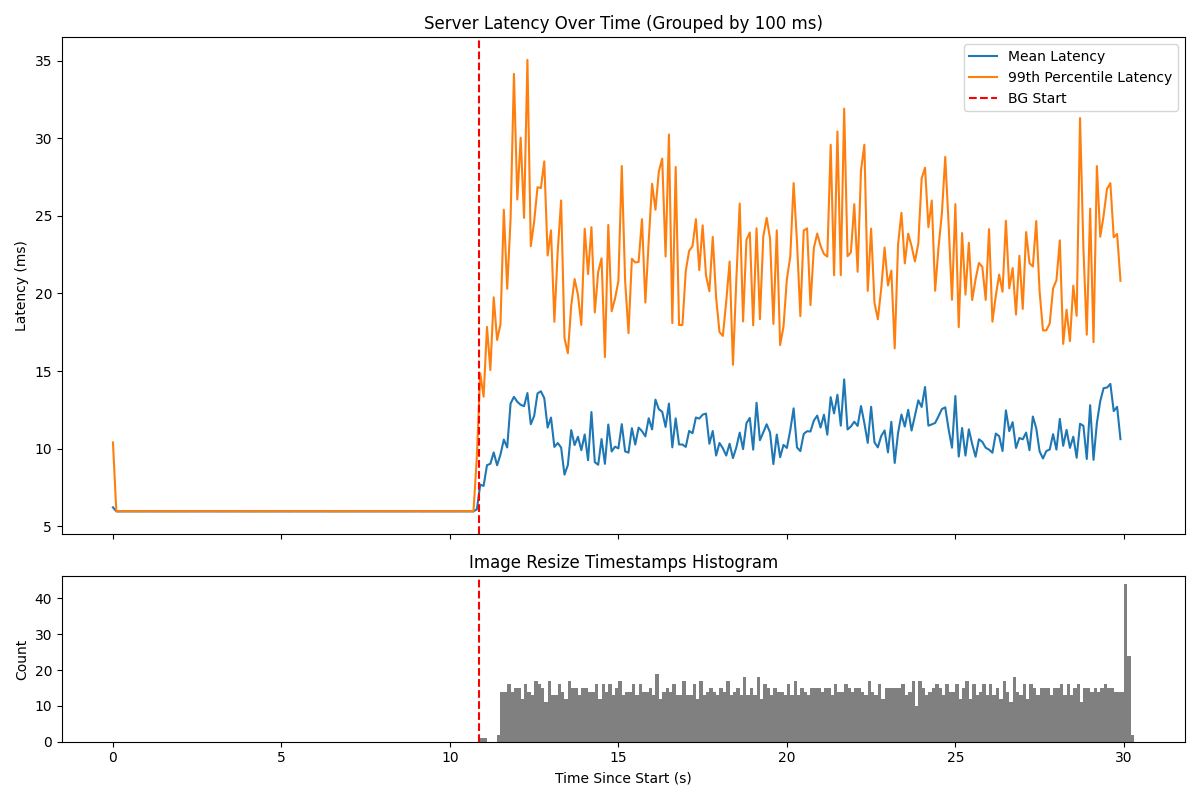
\includegraphics[width=\textwidth]{graphs/unedited-weight-low-two.png}
        \caption{Low load stetting}\label{fig:unedited-weight-low-two}
    \end{subfigure}
    \hspace{\fill}
    \begin{subfigure}[t]{0.48\textwidth}
        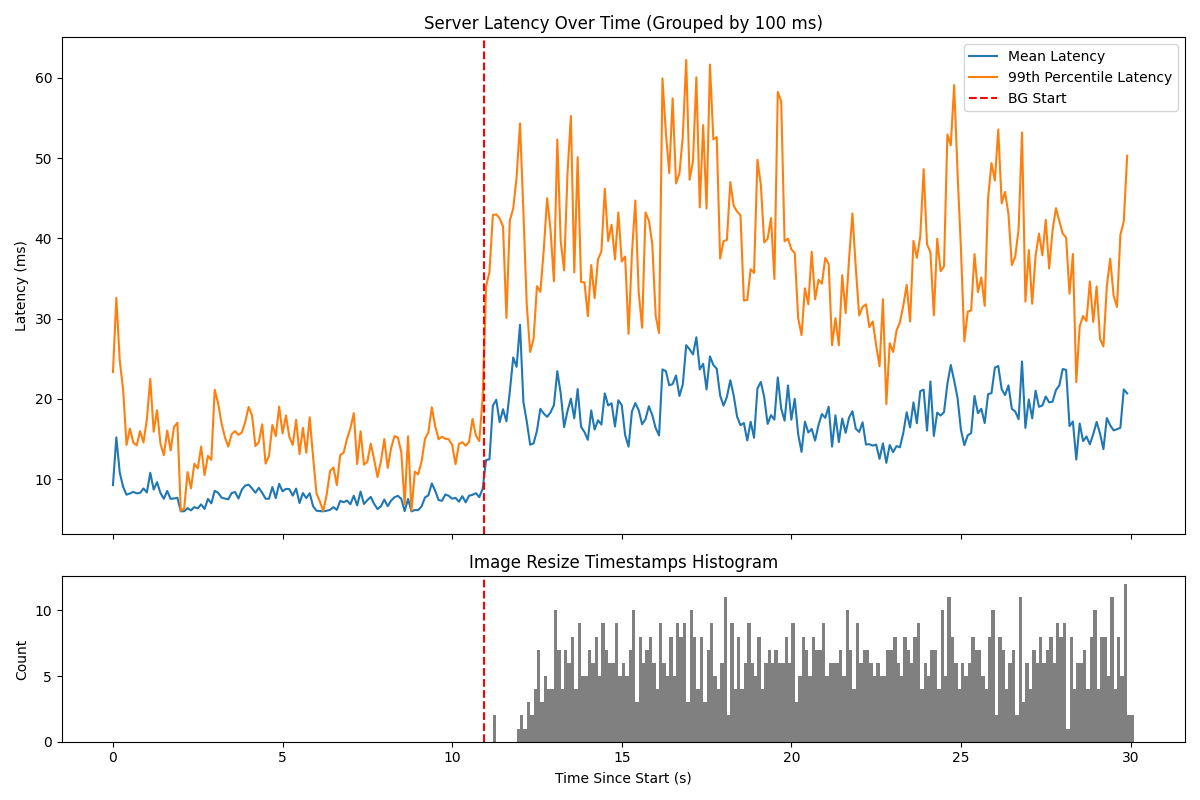
\includegraphics[width=\textwidth]{graphs/unedited-weight-high-two.png}
        \caption{High load setting}\label{fig:unedited-weight-high-two}
    \end{subfigure}
    \caption{Latencies of the server and iteration counts of the background
    tasks in different load scenarios. Note the different y axis limits. The
    upper graphs show end-to-end request latencies, and the bottom graph is a
    histogram of completed iterations of the BE tasks}\label{fig:unedited-weight}
\end{figure*}

In an experiment, we run a (LC) server that processes requests coming in from an
open loop client, running on a separate machine. The client has 100 connections
to the server, each connection creates a new server thread that reads from the
socket and synchronously processes requests in a tight loop. The server threads
run in a cgroup with the highest possible weight: 10000. The server initially
runs on an uncontended four cores, during which time the cpu utilization of the
server is around 85\%. After $\sim$10 seconds, we start two background tasks on
the same four cores, each performing an image resize job. Each background task
is in its own cgroup, which both have the lowest possible weight, 1. We then
measure the latencies experienced by the LC server, before and after starting
the background tasks. Figure~\ref{fig:unedited-weight-low-two} shows the
results. We see that mean latencies spike up from steady at just under 6ms to as
high as 13ms, and much higher for 99th percentile latencies.

With a higher baseline load for the LC server the spikes are higher,
figure~\ref{fig:unedited-weight-high-two} shows the latencies when the
utilization of the uncontended server load is around 95\%.
% .tex extension is presumed

\chapter{Why}



In order to understand why this is happening, we examine a trace of the
experiment. We use schedviz~\cite{schedviz}, a tool that visualizes perf traces,
to examine the scheduling decisions Linux is making.

\begin{figure*}[t]
    \centering
    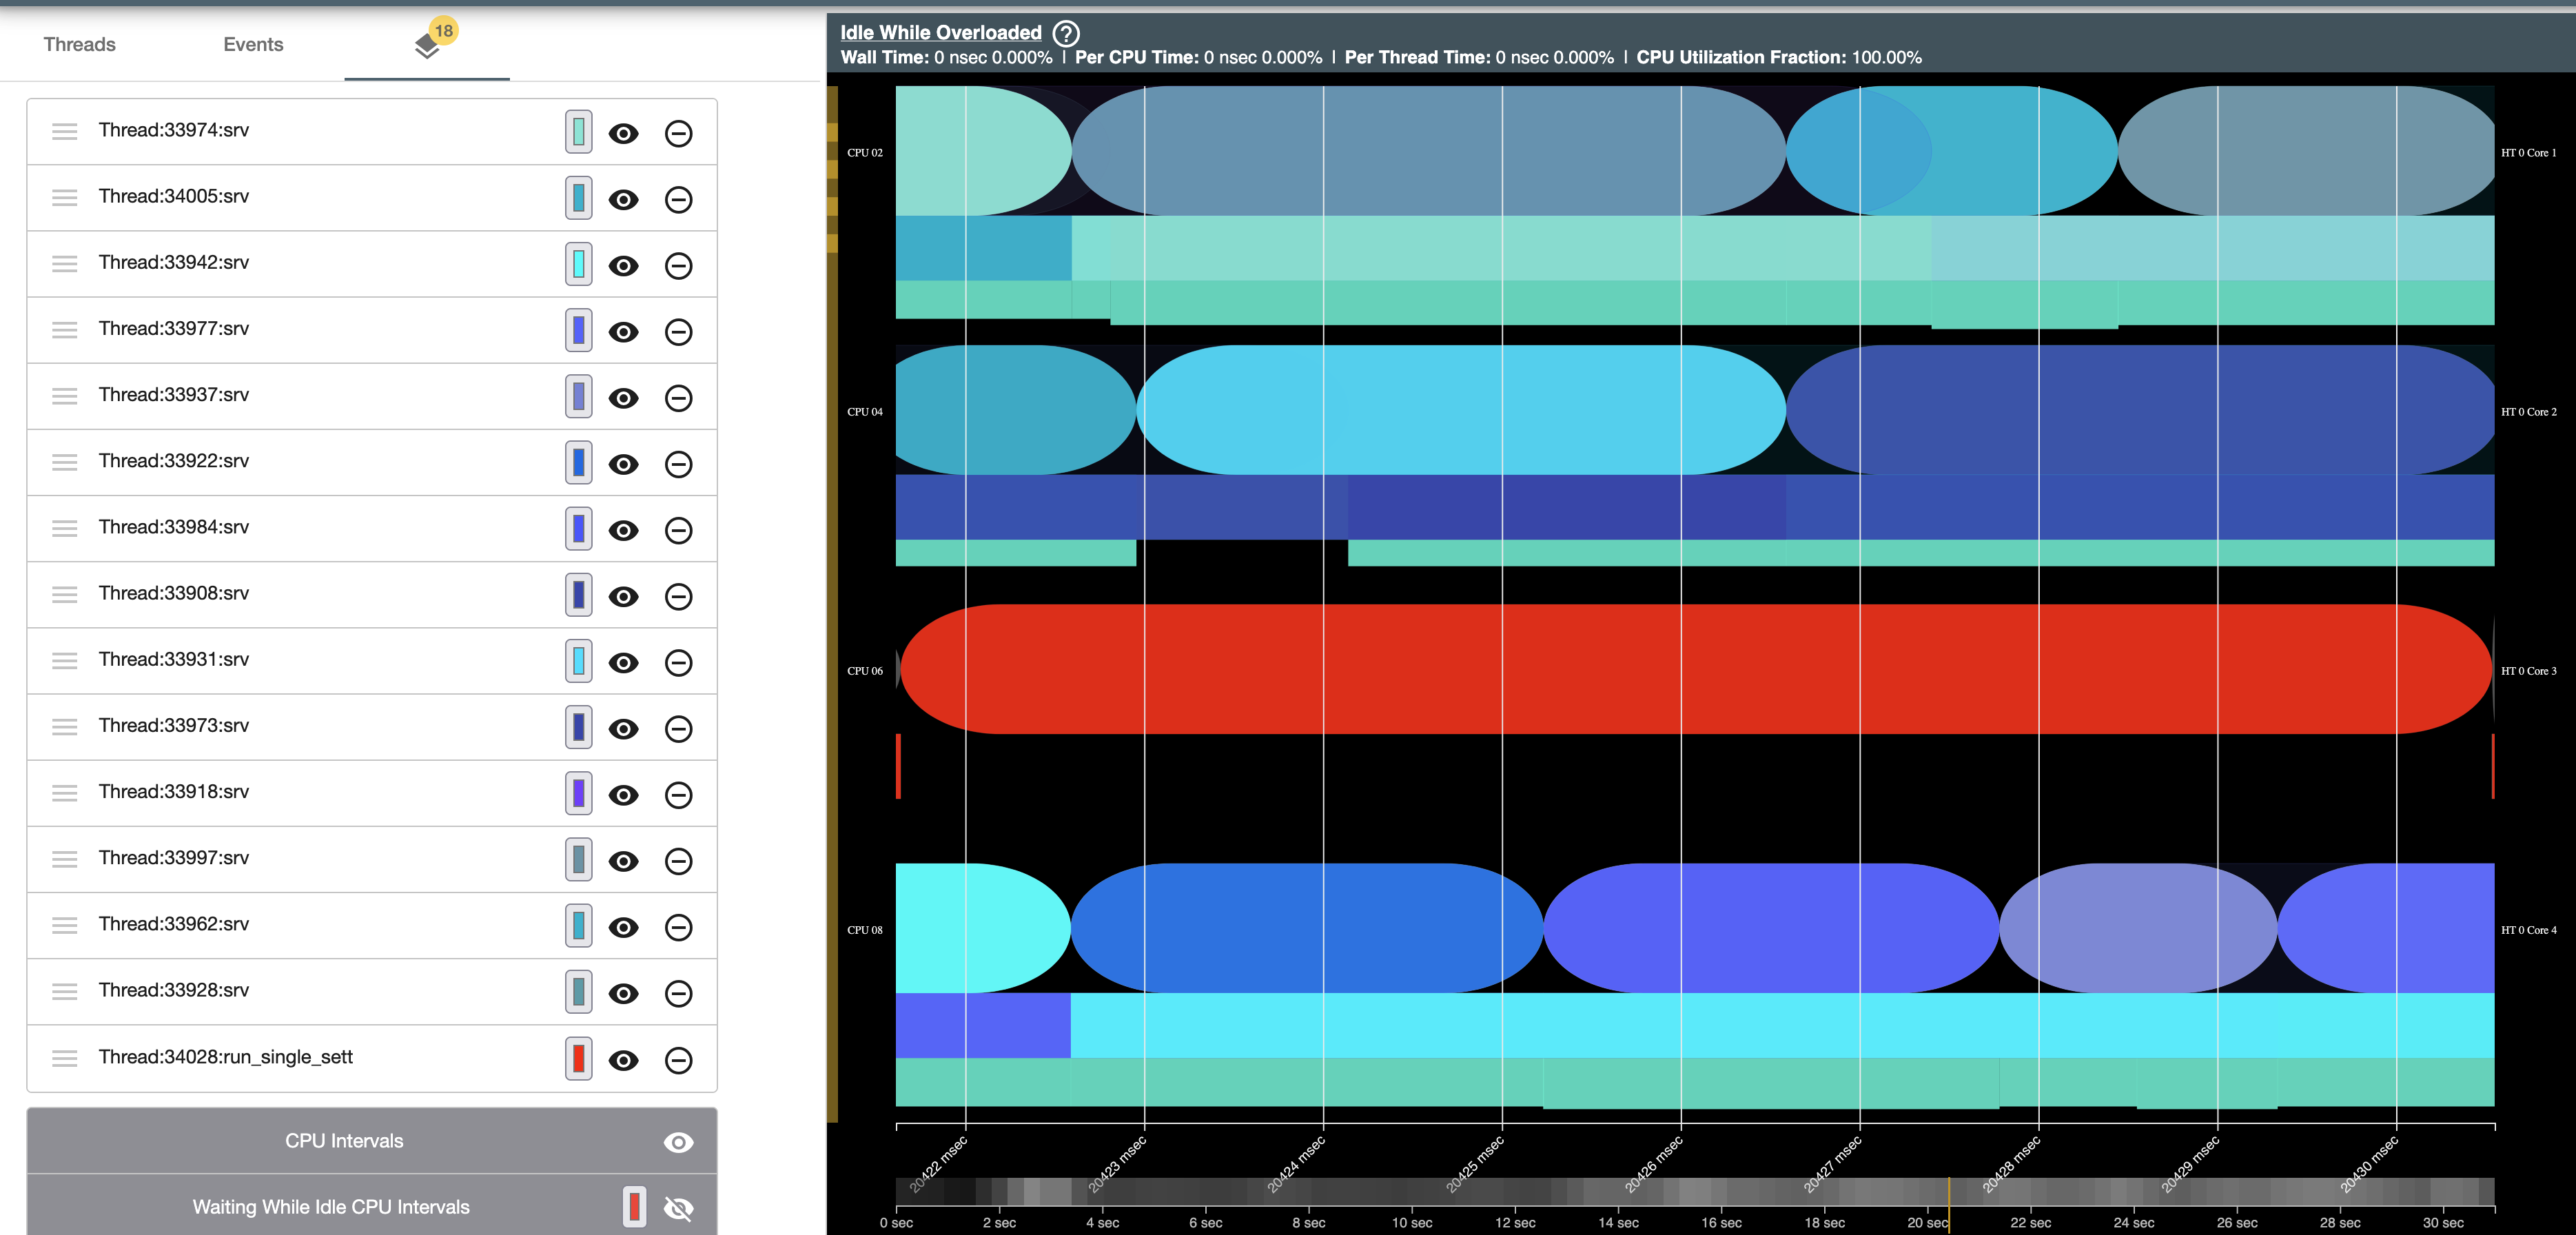
\includegraphics[width=\textwidth]{graphs/schedviz.png}
        \caption{Each thread is a different color. Circles represent which
    thread is running on that core, while rectangles underneath show waiting but
    runnable threads. Core numbers are 2,4,6,8 because this was run on a NUMA
    node so those are the cores that are closest to each other
    }\label{fig:schedviz}
\end{figure*}

In figure~\ref{fig:schedviz}, we look at a 10ms outtake from one of the runs,
that shows the problem occurring. The undesirable behavior we see here is that,
on core 6, the red process that is running the whole time is a BE process. All
the active server threads, shown in varying shades of blue, are on the other
cores, running and, more importantly, waiting.

The reason this happens is that Linux maintains a separate runqueue on each
core. This avoids the synchronization overheads of accessing global state for
every scheduling, but also means that the weight is only strictly enforced
within the individual runqueues, ie within each core. This leads to the depicted
failure mode, where an LC task is waiting on one core while another runs a BE
task.

% \hmng{should I also mention the giving at minimum 4ms? and how that can impact
%  tail latency}


\chapter{Real time scheduling}

There is a way to configure tasks so that Linux enforces global priorities:
processes that run in real time have strict priority over other processes, and
are under a different scheduler that enforces strict and global priorities among
the real time threads.

Linux implements real time scheduling alongside the usual weighted fair share by
supporting different \textit{scheduling classes}. There are three scheduling
classes that are accessible to users, listed in descending order of priority:
Deadline, Fifo, and Normal. Generally speaking most load is expected to fall
into the Normal scheduling class (hence the name). It is the default scheduling
class, and it is only within the Normal scheduling class that the cgroup
cpu.weight interface is relevant.

Each scheduling class exists completely separately: classes maintain their own
run queues and per-entity state; implement their own scheduling algorithms to
choose from the entities on their runqueue; and balance the load across
runqueues on different cores.

Linux isolates strictly between different scheduling classes: it only schedules
a lower scheduling class if the higher scheduling classes found nothing to run,
and each scheduling class tries to steal work from other cores before returning
that it has nothing to run. It is thereby true that if something in the Normal
scheduling class is running, it means there are no Fifo tasks waiting to run
anywhere on the machine.

This global enforcement is not succeptible to the 4ms granularity. This is
because Linux is also able to schedule at other points in time, not just the 4ms
hardware ticks. These occur when the control flow is in the kernel anyway, and
include the \textit{exit} path, when the running thread blocks, and
\textit{entry}, when a sleeping thread is woken up (via a separate signal, for
example receiving a packet on a listening socket). In these contexts Linux is
able to make fast scheduling decisions, and scheduling at these events is
sufficient to enforce isolation: the tick-based preemption granularity is
relevant for latencies of the processes within a priority, but isolating across
priorities only requires the correct scheduling decision to be made on entry and
exit. 

\begin{figure*}[t]
    \centering
    \begin{subfigure}[t]{0.48\textwidth}
        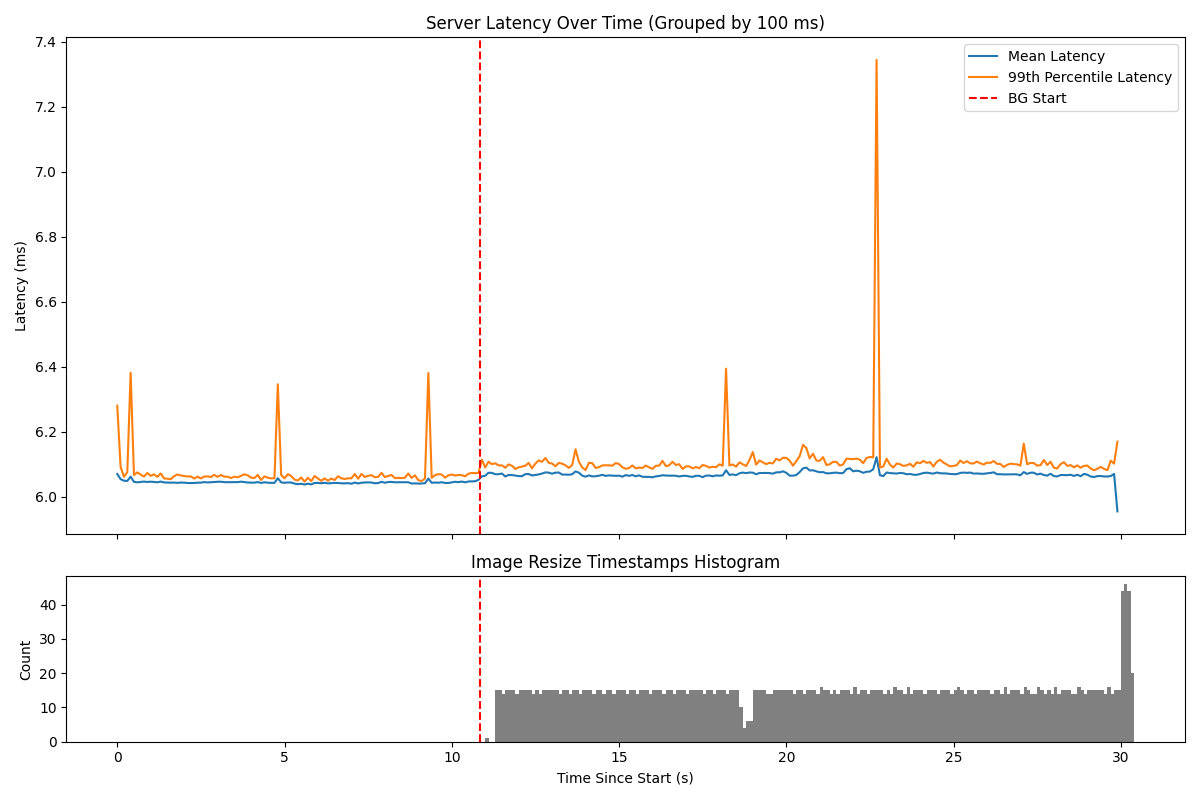
\includegraphics[width=\textwidth]{graphs/unedited-rt-low-two.png}
        \caption{Low load}\label{fig:unedited-rt-low-two}
    \end{subfigure}
    \hspace{\fill}
    \begin{subfigure}[t]{0.48\textwidth}
        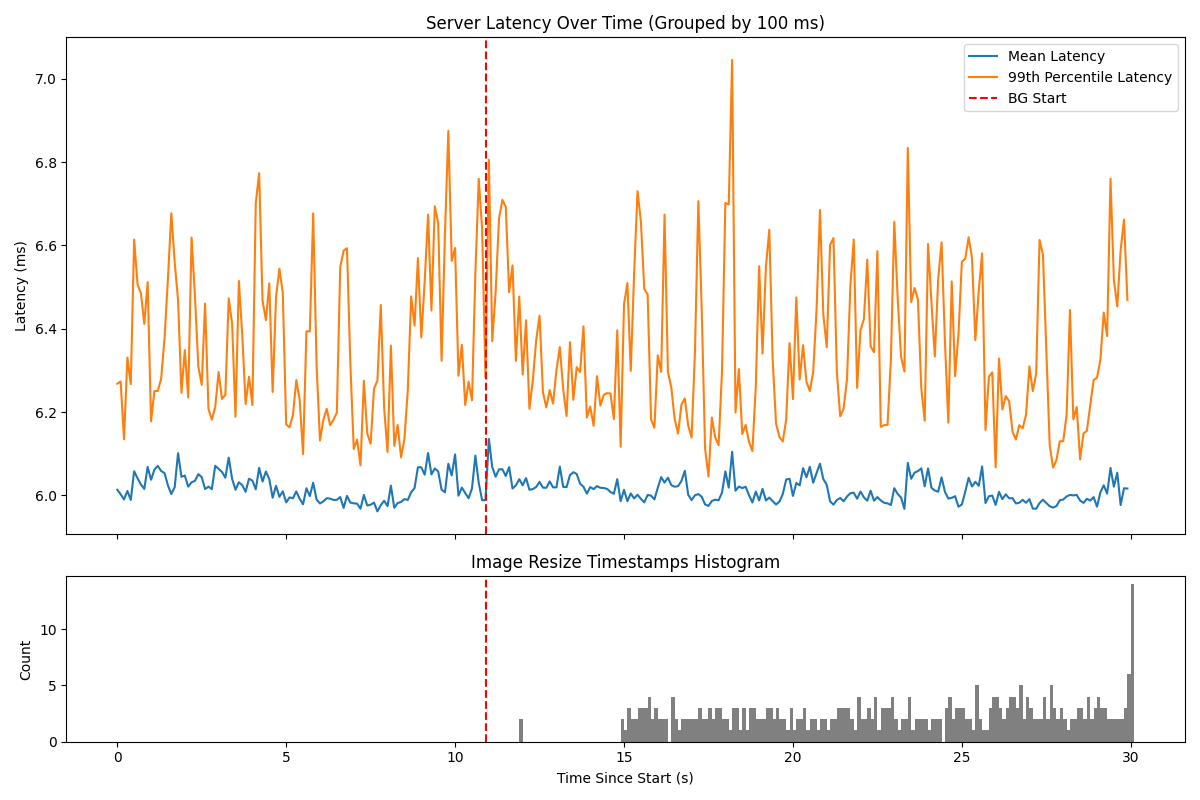
\includegraphics[width=\textwidth]{graphs/unedited-rt-high-two.png}
        \caption{High load}\label{fig:unedited-rt-high-two}
    \end{subfigure}
    \caption{Results of the same experiment, with LC running as a real time process}\label{fig:unedited-rt}
\end{figure*}

This points to a possible solution: run LC in Fifo and BE in Normal. Doing so
effectively promotes the latency criticality of the LC task in the eyes of the
system, and makes use of Linux's strong isolation of real time workloads.
Figure~\ref{fig:unedited-rt} shows the resulting measured latencies in the same
low and high load setting as previously. We see much stabler latencies, as
expected; in the baseline as well as once the BE tasks are started. This looks
promising on two fronts: 1: we get better isolation by making use of Linux's
strict boundaries between scheduling classes, and 2: we see improved tail
latency for the LC task by using a fifo run-to-completion scheduling algorithm.

However, the first benefit of improved stability comes at a cost. Because the
global ordering is so strict, also within the Fifo scheduling class, Linux is
performing balancing and potentially migration almost every time an LC thread
wakes up or exits. This requires the scheduling core to potentially lock the
runqueues of all the other cores as it ensures the task it will run the next is
the one with the highest priority, and within that priority the once that first
became runnable. This increase in scheduling latency leads to the small increase
in the baseline latency that is visible in the graphs.

And second benefit, the observed improved tail latency, is a side-effect of the
experimental setup, where each request does the exact same thing and processing
times are uniform. This is not true for a production environment, where request
processing times are variable and unknown. If a fifo run-to-completion scheduler
is used in that setting, it leads to HoL blocking, and thus to much worse tail
latencies for short requests.

We conclude that the Fifo scheduling class is not a good solution: although it
is able to globally ensure isolation between LC and BE tasks, its scheduling
time overheads and algorithm make in poorly suited for a production setting.





\chapter{Half a scheduling class}\label{chp:sched_idle}

% \hmng{transition??}
Within the Normal scheduling \textit{class}, Linux supports two different
scheduling \textit{policies}: \schednormal{} and \schedidle{}, where
\schednormal{} is the default. Under the hood, the scheduler for the Normal
class keeps the tasks of both policies on the same runqueue, and they are all
scheduled using the same algorithm. Thus, \schedidle{} is in principle not very
different from just being a low-weight process: From the scheduler's
perspective, \schedidle{} entities are just entities with a predefined low
weight (currently 3). There is, confusingly, also and Idle scheduling
\textit{class}, but that not accessible to userspace and exists solely to manage
the core's transition in and out of being actually idle (ie running nothing).

The main way that \schedidle{} entities are special-cased from \schednormal{}
entities is during wakeup: in 2019 a patch to Linux\cite{fixing-sched-idle-lwn}
added a check where, when a \schednormal{} entity becomes newly runnable, if the
core where the entity is waking up is already running something in
\schednormal{}, it will look for other cores that might be currently running a
\schedidle{} entity, and migrates the new entity there.

In doing so, Linux created a half scheduling class. In order to implement fully
invariant that no process of category B is ever running if a task of category A
is queued, that requires 1: checking if other cores are running a B task when an
A task wakes up on a core already running an A task, and 2: checking if another
core has a queued A task before running a B task.\ \schedidle{} does step 1, but
not step 2.

\schedidle{} is also promising because it was extended to have cgroup support
recently\cite{cgroup-idle-patch}: when set via the cpu.idle cgroup interface
file, the entire cgroup is counted as a \schedidle{} entity.

\begin{figure*}[t]
    \centering
    \begin{subfigure}[t]{0.48\textwidth}
        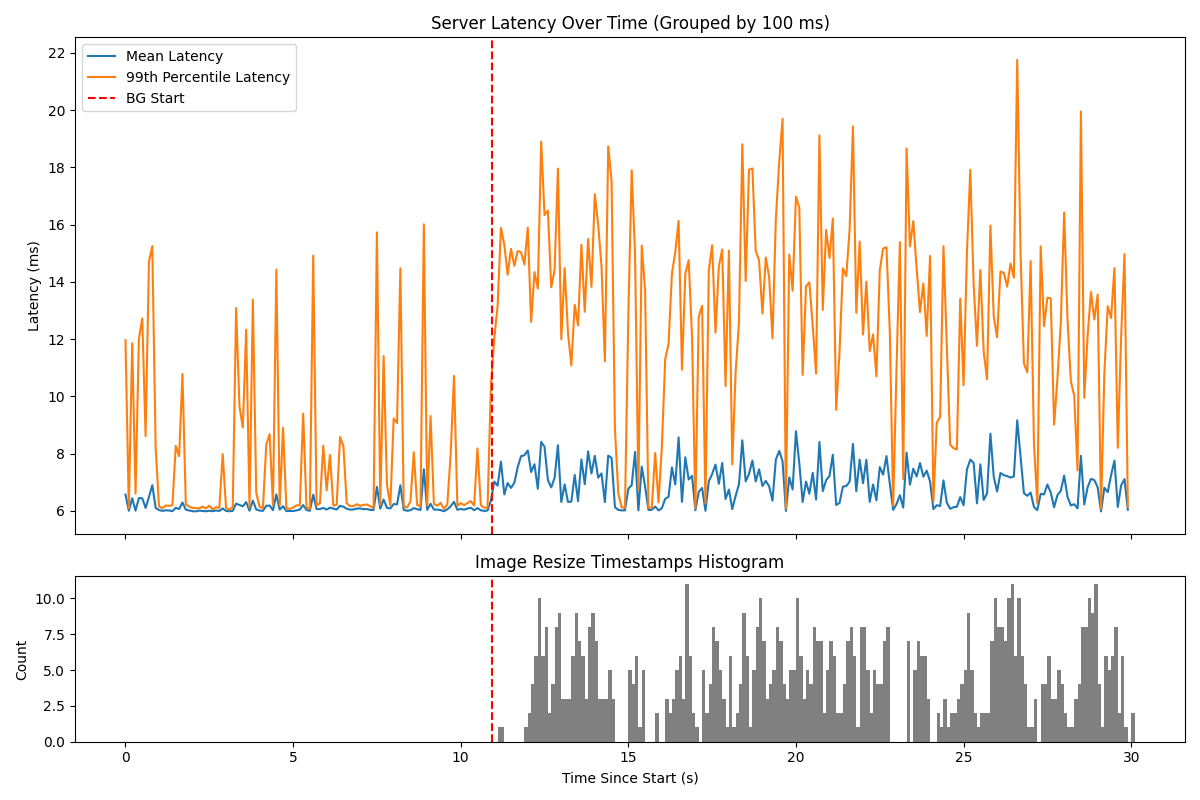
\includegraphics[width=\textwidth]{graphs/unedited-idle-low-two.png}
        \caption{Low load}\label{fig:unedited-idle-low-two}
    \end{subfigure}
    \hspace{\fill}
    \begin{subfigure}[t]{0.48\textwidth}
        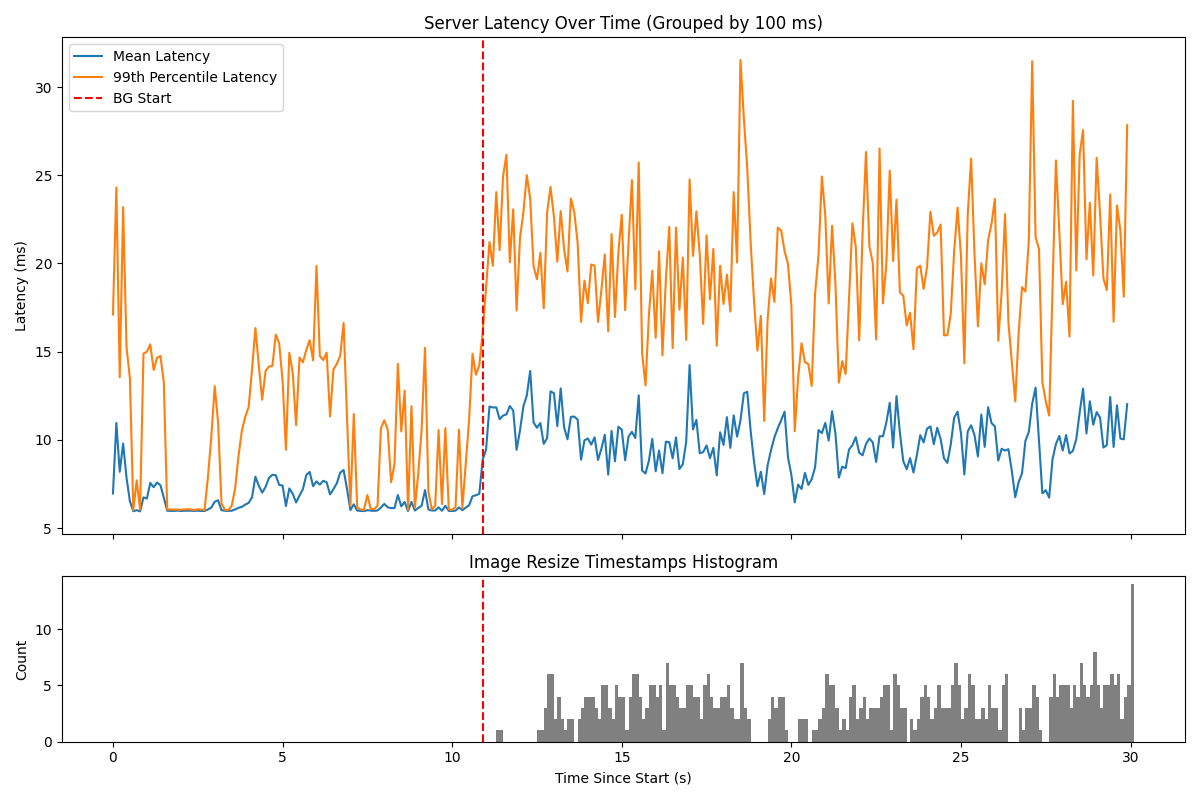
\includegraphics[width=\textwidth]{graphs/unedited-idle-high-two.png}
        \caption{High load}\label{fig:unedited-idle-high-two}
    \end{subfigure}
    \caption{using \schedidle{}}\label{fig:unedited-idle}
\end{figure*}

And indeed, we find that when we use cgroups' new cpu.idle interface feature,
the latency impact of the BE tasks decreases, although it does not entirely drop
to what we saw with the Fifo class. Figure~\ref{fig:unedited-idle} shows the
results, for the familiar settings of low and high load. The jump we see in the
mean latency has decreased from peaks as high as 13ms to around 7ms (even though
in principle they now have a higher weight).




\chapter{Making it whole}

The performance of the current \schedidle{} policy shows us that if we want to
completely isolate LC and BE, we need to put in the final piece to make
\schedidle{} effectively its own scheduling class.

We write a Linux patch that does this. The patch intervenes in two places in the
current scheduling process: 1: it ensures that no \schedidle{} entity will be
chosen if there is a runnable \schednormal{} entity (this overrides the fair
share that even a weight 1 process would occasionally get in unmodified kernel),
and 2: it tries to steal queued \schednormal{} entities from other cores before
running a \schedidle{} entity.

\begin{figure*}[t]
    \centering
    \begin{subfigure}[t]{0.48\textwidth}
        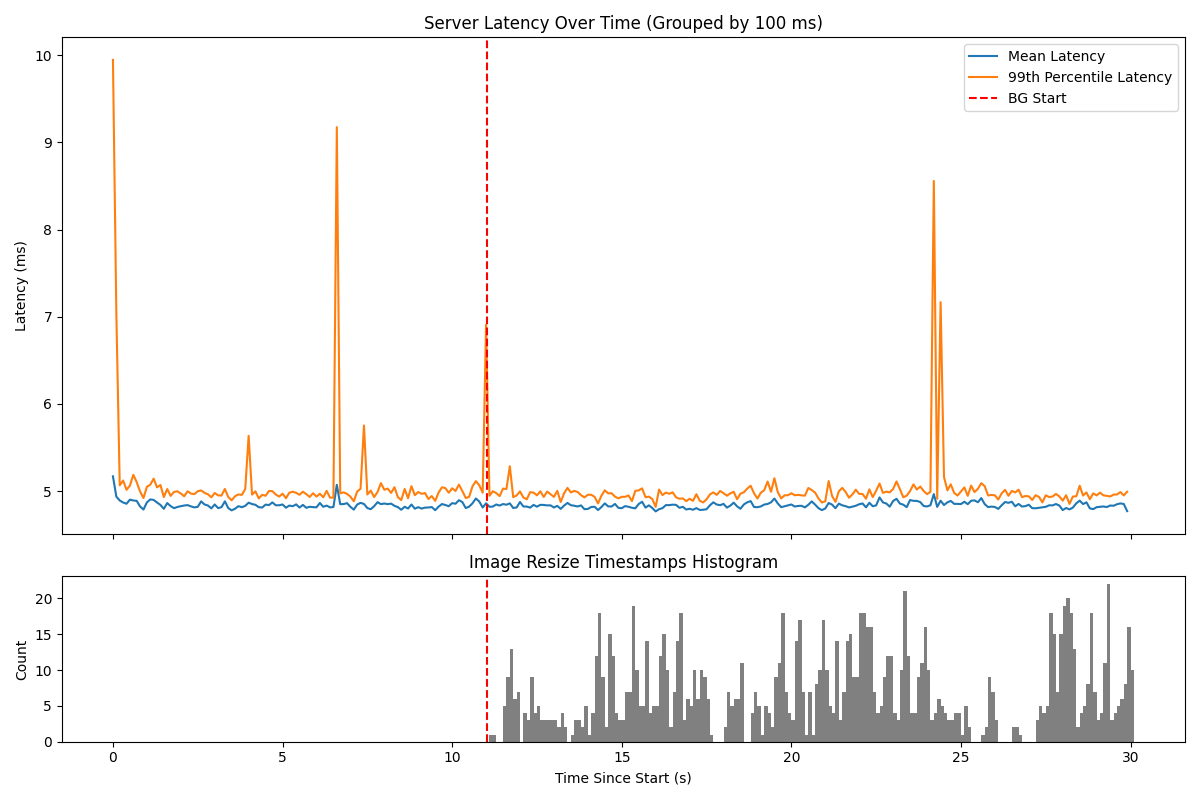
\includegraphics[width=\textwidth]{graphs/patched-idle-low-two.png}
        \caption{Low load}\label{fig:patched-idle-low-two}
    \end{subfigure}
    \hspace{\fill}
    \begin{subfigure}[t]{0.48\textwidth}
        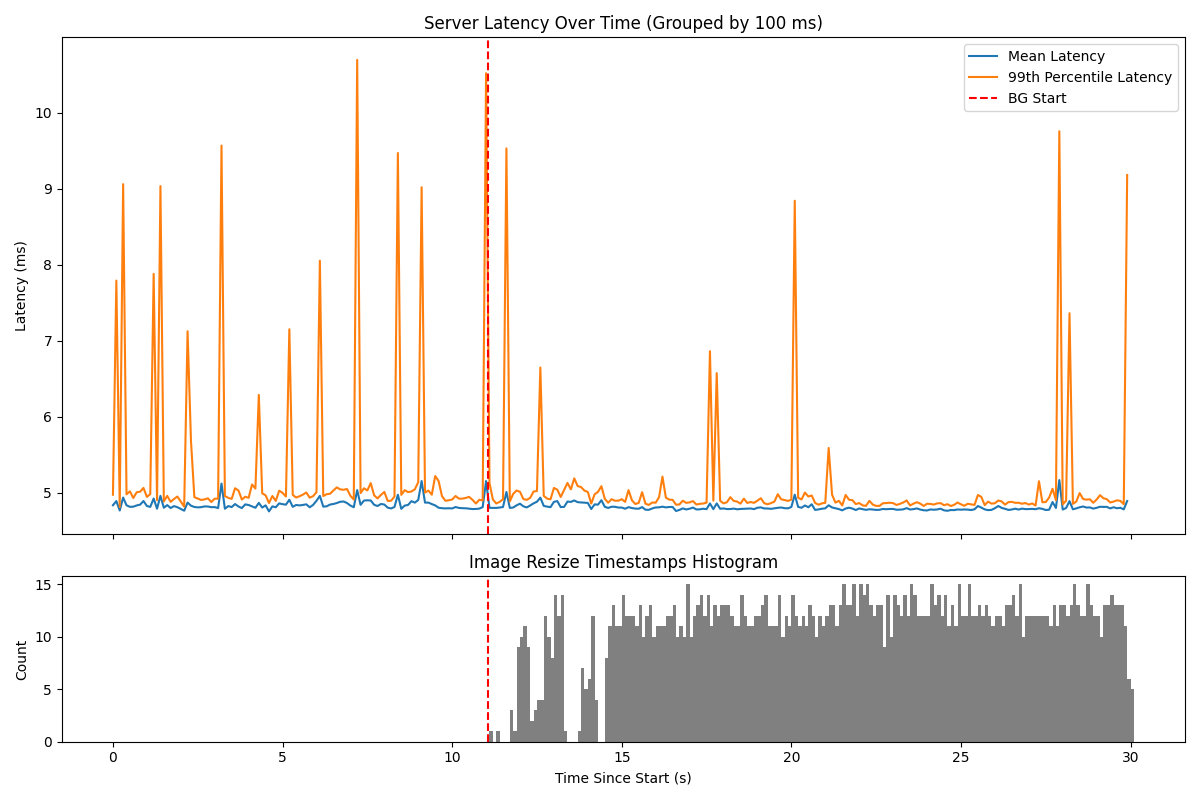
\includegraphics[width=\textwidth]{graphs/patched-idle-high-two.png}
        \caption{High load}\label{fig:patched-idle-high-two}
    \end{subfigure}
    \caption{using a patched \schedidle{} that steals queued \schednormal{}
    tasks before running \schedidle{} ones}\label{fig:patched-idle}
\end{figure*}

We can see the resulting performance in figure~\ref{fig:patched-idle}, and see
that as desired the latency of the server remains stable after the background
tasks start. This does not mean that the background task never runs: the lower
graph still shows iterations of image resizing being done. The difference is
that now the background tasks will reliably get interrupted when the LC server
has a request to process.




%%% Appendicies of thesis  %%%%%%%%%%%%%%%%%%%%%%%%%%%%%%%%%%%%%%%%%%%%%%%%%%%%%%%%%%%%%%%%%%%%%%%%

\appendix
% From mitthesis package
% Version: 1.01, 2023/07/04
% Documentation: https://ctan.org/pkg/mitthesis


\chapter{Code listing}

This example uses the \texttt{listings} package.

\bigskip

\lstdefinestyle{mystyle}{
    backgroundcolor=\color{CadetBlue!15!white},   
    commentstyle=\color{Red3},
    numberstyle=\tiny\color{gray},
    stringstyle=\color{Blue3},
    basicstyle=\small\ttfamily,
    breakatwhitespace=false,         
    breaklines=true,                 
    numbers=left,                    
    numbersep=5pt,                  
    showspaces=false,                
    showstringspaces=false,
    showtabs=false,                  
    tabsize=2
}%
\lstset{language=[5.3]Lua,style={mystyle}}%

\begin{lstlisting}
function print_rate(kappa,xMin,xMax,npoints,option)
     local c = 1-kappa*kappa
     local croot = (1-kappa*kappa)^(1/2)
     local logx = math.log(xMin)
     local psi = 0
     
     local xstep = (math.log(xMax)-math.log(xMin))/(npoints-1)
     
     arg0 = math.sqrt(xMin/c)
     psi0 = (1/c)*math.exp((kappa*arg0)^2)*(erfc(kappa*arg0)-erfc(arg0))
     
     if option~=[[]] then
  		 tex.sprint("\\addplot+["..option.."] coordinates{") 
  		 -- addplot+ for color cycle to work
     else
  		 tex.sprint("\\addplot+ coordinates{")
     end
     tex.sprint("("..xMin..","..psi0..")")
     
     for i=1, (npoints-1) do
  		 x = math.exp(logx + xstep)
  		 arg = math.sqrt(x/c)
  		 karg = kappa*arg
  		 if karg<5 then 
		 -- this break compensates for exp(karg^2), which multiplies the error in the erf approximation...
  		    logpsi = -math.log(croot) + karg^2 + math.log(erfc(karg)-erfc(arg))
  		    psi = math.exp(logpsi)
  		 else
  		    psi = (1/(karg) - 1/(2*(karg^3)) + 3/(4*(arg^5)) )/(1.77245385*croot)
  		    -- this is the large x asymptote of the reaction rate
  		 end
  		 logx = math.log(x)
  		 tex.sprint("("..x..","..psi..")")
     end
     tex.sprint("}")
end
\end{luacode*}
\end{lstlisting}
% listings example


%%% Bibliography (biblatex)  %%%%%%%%%%%%%%%%%%%%%%%%%%%%%%%%%%%%%%%%%%%%%%%%%%%%%%%%%%%%%%%%%%%%%%

\defbibheading{bibintoc}{\chapter*{#1}\addcontentsline{toc}{backmatter}{\refname}} 
% this sets the title of contents name for bibliography to \refname (= References)
% change "backmatter" to "chapter" if you prefer a bold face entry in the table of contents

\printbibliography[title={\refname},heading=bibintoc]

% biblatex also supports chapter-by-chapter bibliography, https://tex.stackexchange.com/a/296502/119566
% see the biblatex manual, section 3.14.3


\end{document} 
 